\documentclass[11pt]{article}
%\usepackage{psfig}
\usepackage{graphicx}
\usepackage{enumitem}
\usepackage{amsmath,amssymb,amsthm,listings,hyperref}
\usepackage{tikz}
\usepackage{latexsym}
\usepackage{amsfonts}

\title{CS 4641 Project 4 Report}
\author{HU Heng}
\begin{document}
\maketitle
\section{Overview}
This report is for CS 4641 Machine Learning project 4 Markov Decision Process. In the following pages, you will see the solution to the chosen Markov decision process using value iteration, policy iteration and Q learning. I will show the convergence of value iteration and policy iteration as well as the influence of changing PJOG values. Finally, Q learning is discussed.

\section{My MDP Problems}
In this project, I use the RL\_sim which is the java executable created by Carnegie Mellon University associates Rohit Kelkar and Vivek Mehta. The problems I would like to solve are both mazes given by the author. Fig.\ref{Fig:maze1} is a very simple 6x9 maze and Fig.\ref{Fig:maze2} is a more complicated 10x10 maze.
\begin{figure}[!htb]
   \begin{minipage}{0.4\textwidth}
     \centering
     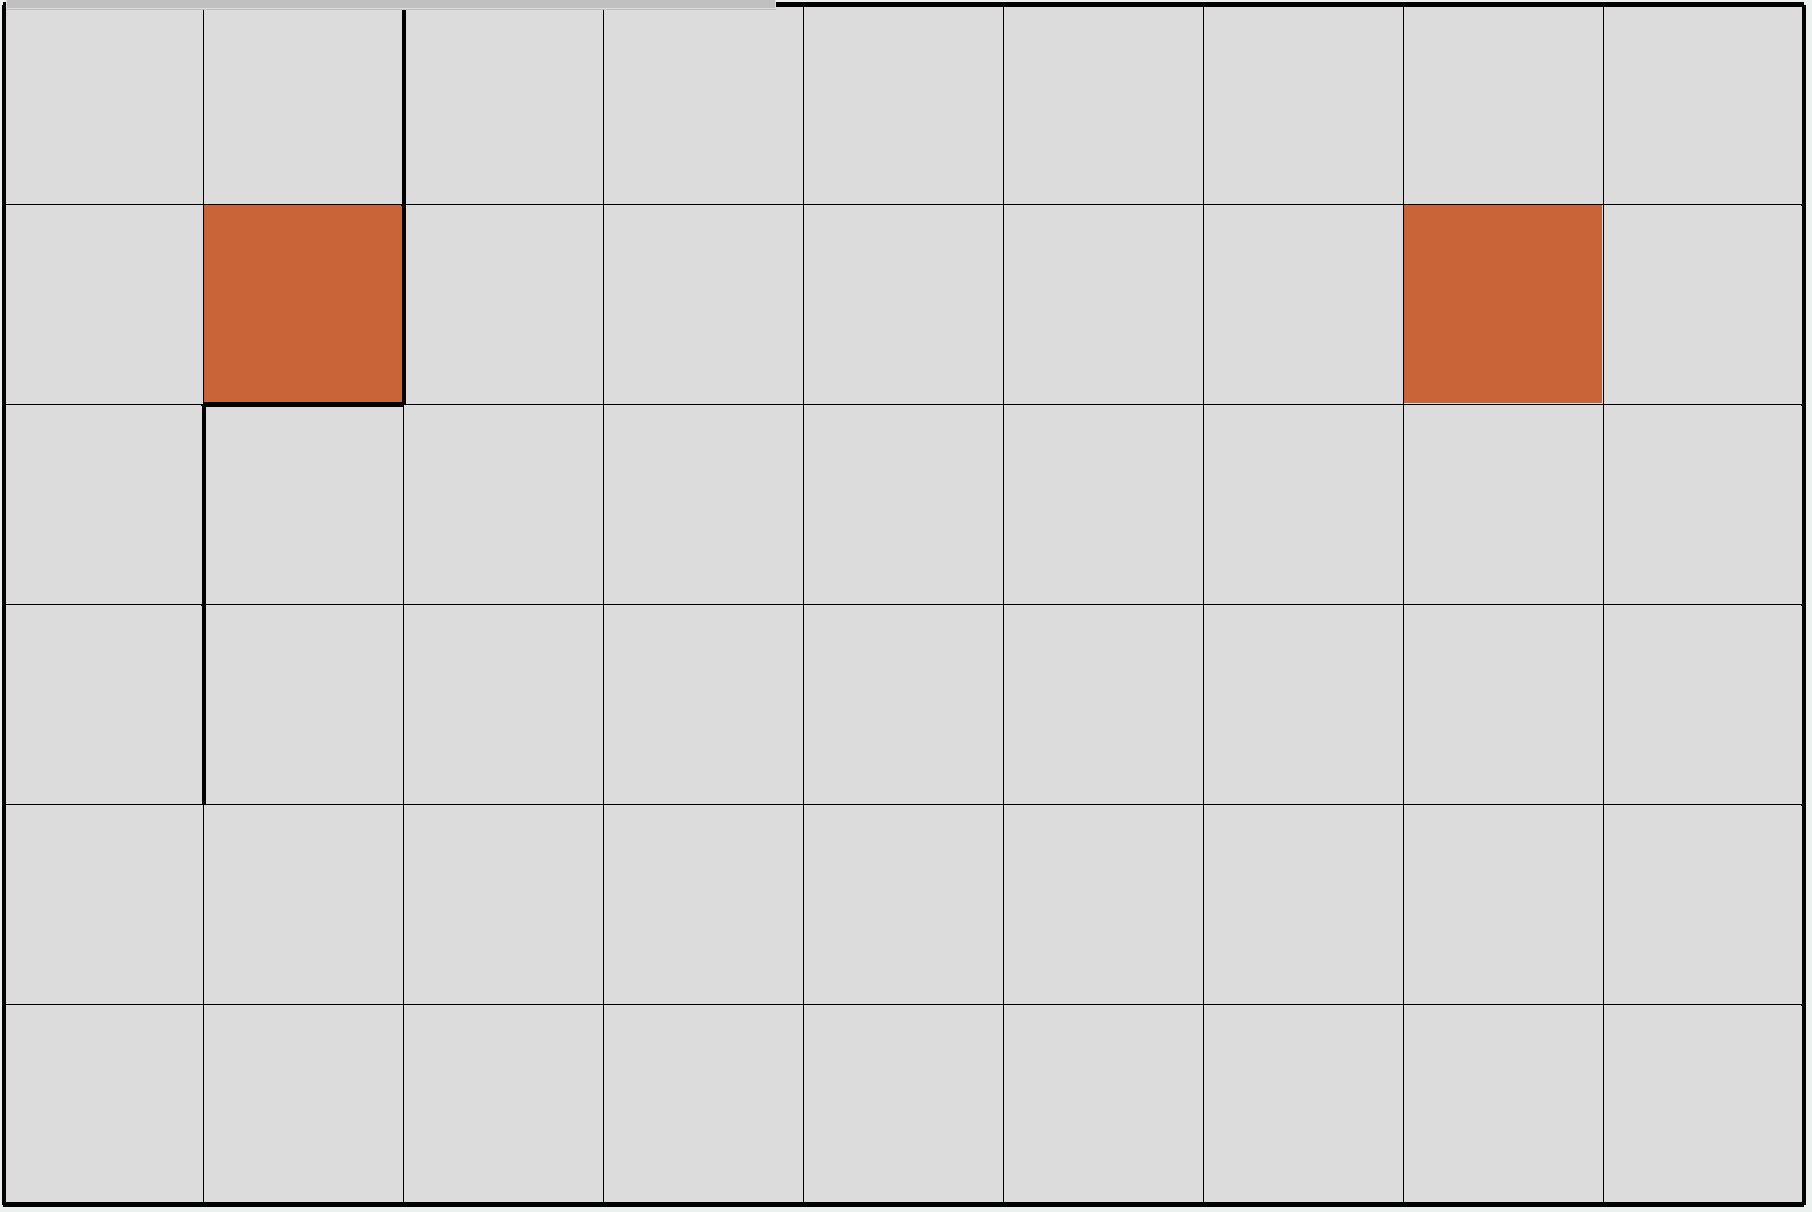
\includegraphics[width=1.2\linewidth]{../figures/maze1.png}
     \caption{Simple Maze}\label{Fig:maze1}
   \end{minipage}\hfill
   \begin{minipage}{0.4\textwidth}
     \centering
     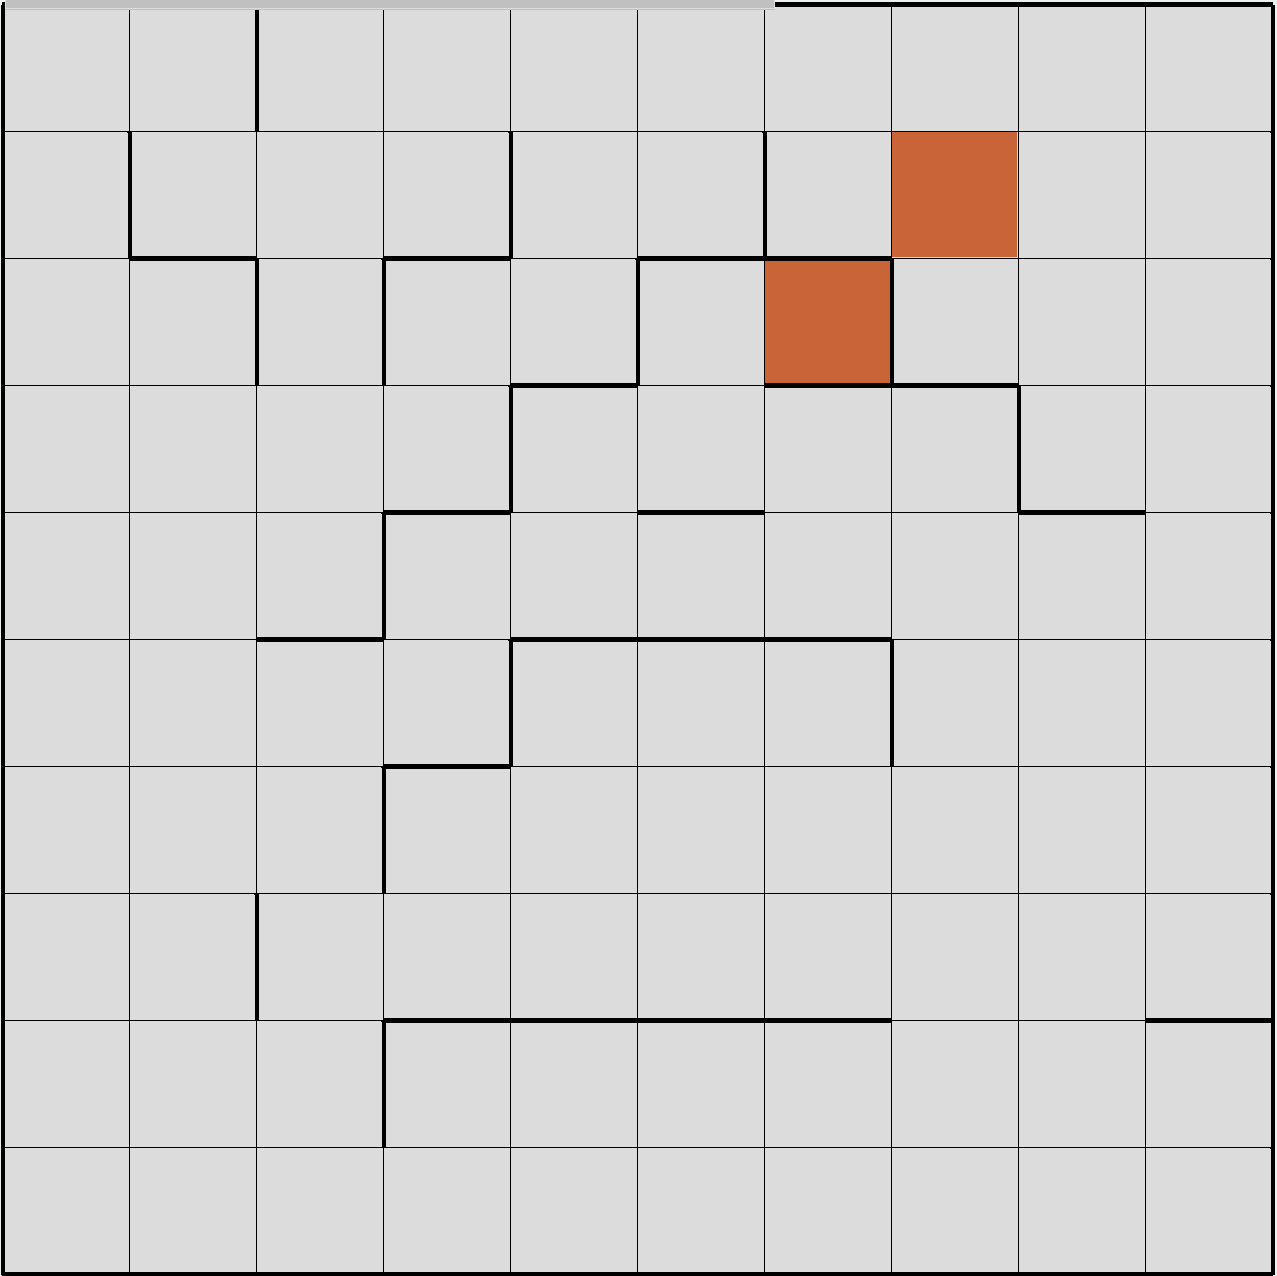
\includegraphics[width=1\linewidth]{../figures/maze2.png}
     \caption{Complex Maze}\label{Fig:maze2}
   \end{minipage}
\end{figure}\\
\\
In the figures, the highlighted grids are the destinations and the bold lines are walls and the agent cannot pass the wall. The possible actions for the agent are moving up, down, right or left and each action will have some constant cost. The parameter PJOG is the probability that the agent will act ineffectively. i.e. the agent will have 1-PJOG probability that its action will lead to the destination and PJOG/3 probability to choose other directions. Also, there would be some penalty if the agent tries to go into a wall.\\
\\
I believe these two problems are interesting. The first reason is that they can be mapped to some real life problems. For example, a robot has to go back to its charging position when its battery is low. Another reason is that I believe the problems can show the performance of different algorithms as well as help the selection of algorithms in different situations.
\section{Value Iteration}
For value iteration, it works by finding the optimal value function which can represent how good is a state for the agent. It will apply the optimal Bellman operator to the value function in a recursive manner and converge to the optimal value. Then, we can get the corresponding optimal policy for every state. \ref{Tab:value} shows the time and steps for value iteration to converge for different selection of PJOG value. Fig.\ref{Fig:value1_1} to Fig.\ref{Fig:value1_5} shows the result of small maze and Fig.\ref{Fig:value2_1} to Fig.\ref{Fig:value2_5} shows the result of large maze.
\begin{table}[h!]
  \begin{center}
    \caption{Performance of Value Iteration}
    \label{Tab:value}
    \begin{tabular}{c|c|c|c|c}
      \textbf{PJOG} & \textbf{Small\_Iterations} & \textbf{Small\_Time(ms)} & \textbf{Large\_Iterations} & \textbf{Large\_Time(ms)}\\
      \hline
      0.1 & 24 & 4 & 42 & 40\\
      0.3 & 48 & 19 & 84 & 65\\
      0.5 & 123 & 23 & 181 & 143\\
    \end{tabular}
  \end{center}
\end{table}\\
\\
From the experiments, we can see that the increase of PJOG will lead to longer run time and steps for value iteration to converge. This is within my expectation because large value of PJOG means the agent will have higher probability to do ineffective actions, that is, a higher chance to waste time. Also, the time and steps increase when we change from small maze to large maze, which is a very trivial result.

\begin{figure}[!htb]
   \begin{minipage}{0.4\textwidth}
     \centering
     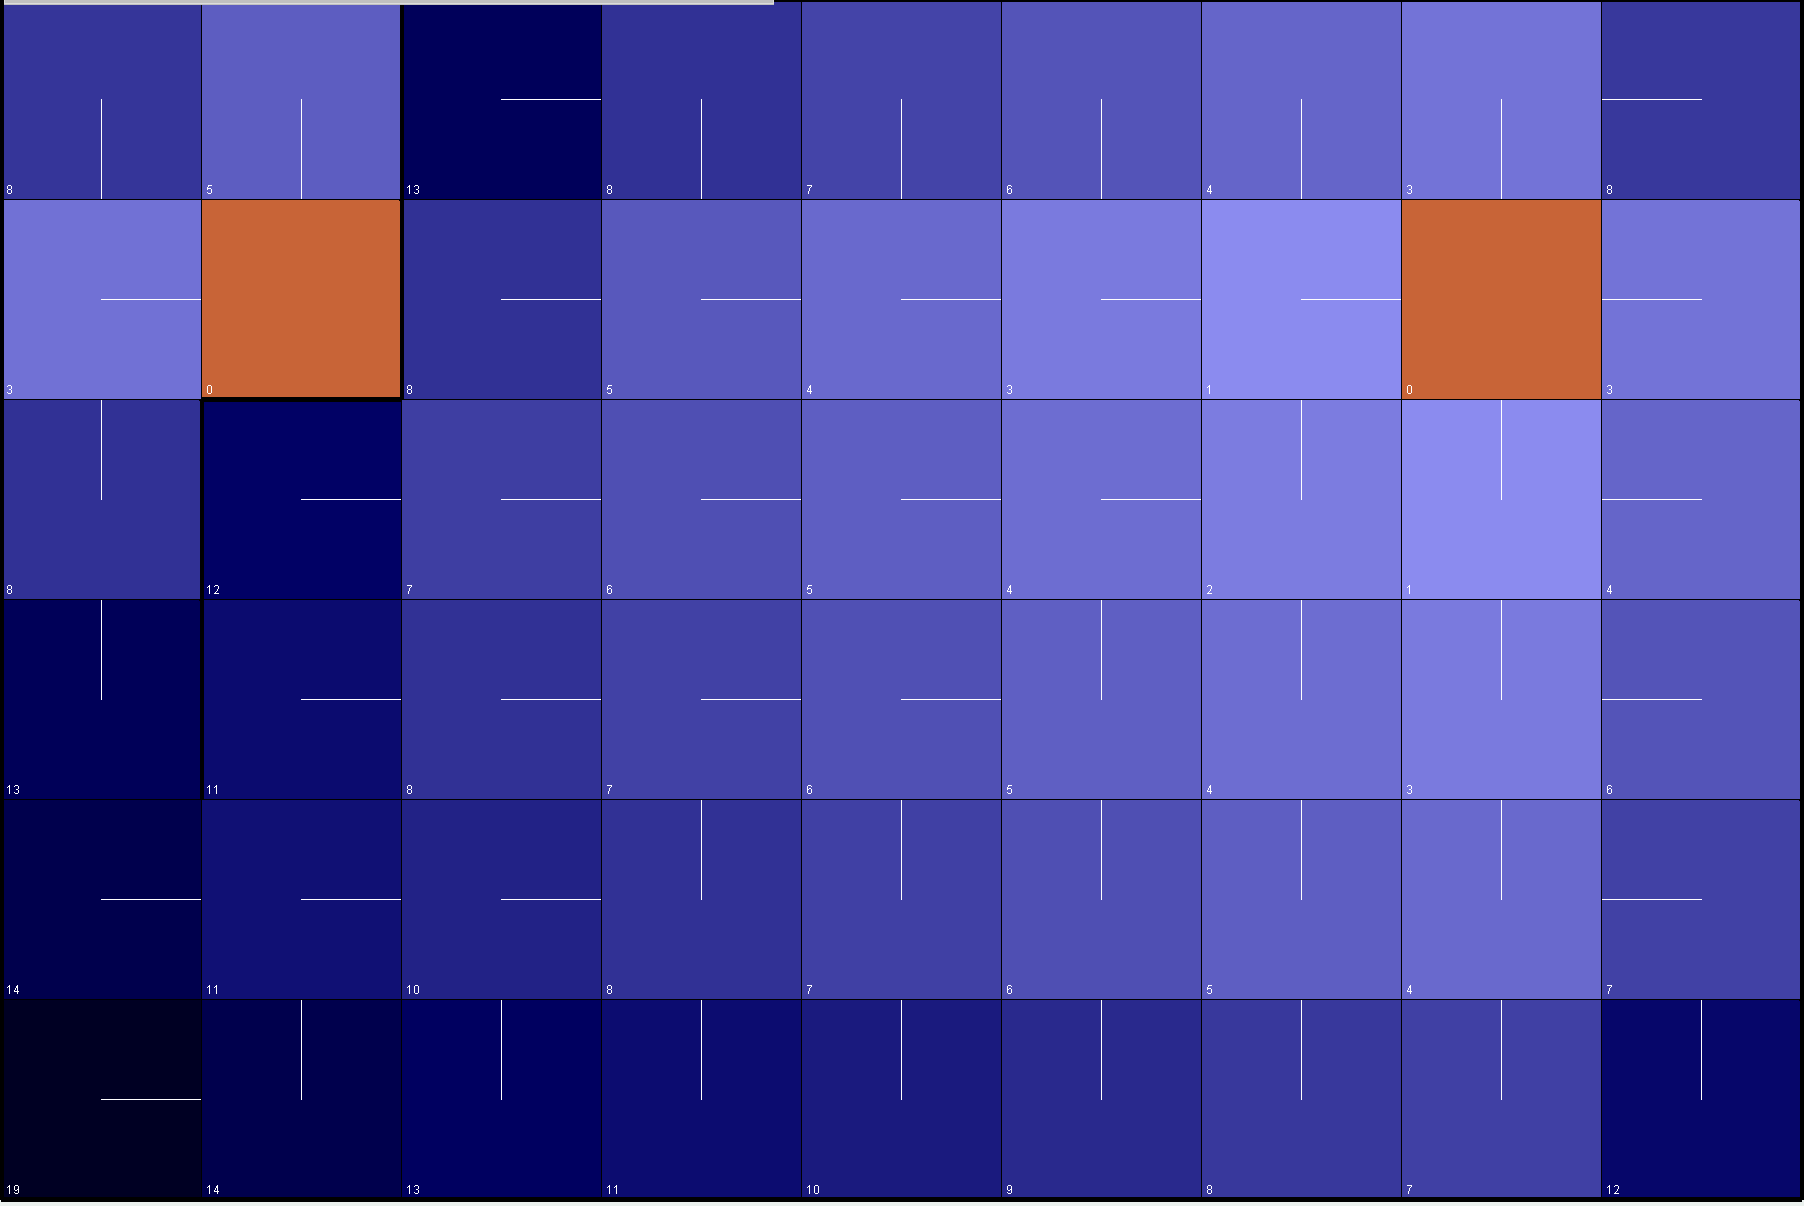
\includegraphics[width=1.2\linewidth]{../figures/value1_1.png}
     \caption{Small Maze, Value Iteration, PJOG=0.1}\label{Fig:value1_1}
   \end{minipage}\hfill
   \begin{minipage}{0.4\textwidth}
     \centering
     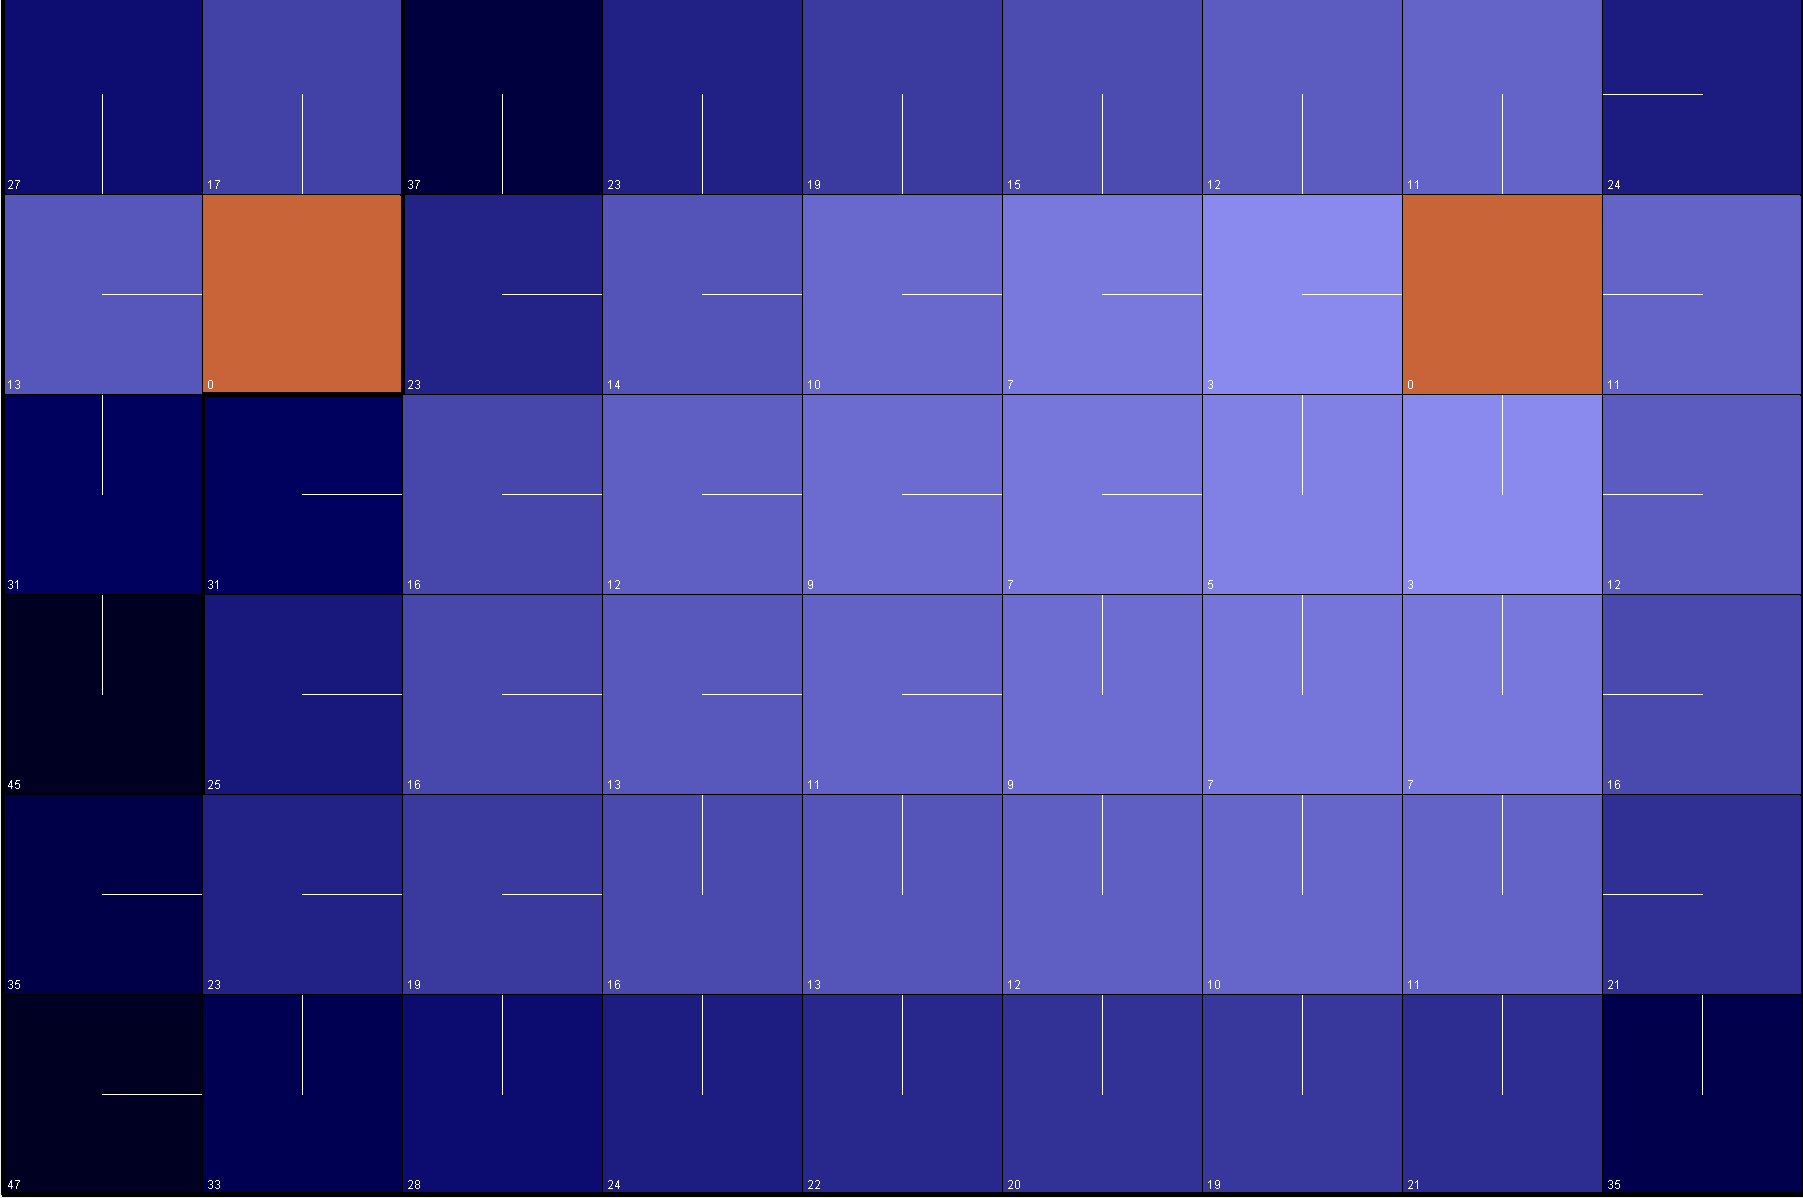
\includegraphics[width=1.2\linewidth]{../figures/value1_3.png}
     \caption{Small Maze, Value Iteration, PJOG=0.3}\label{Fig:value1_3}
   \end{minipage}
\end{figure}

\begin{figure}[!htb]
   \begin{minipage}{0.4\textwidth}
     \centering
     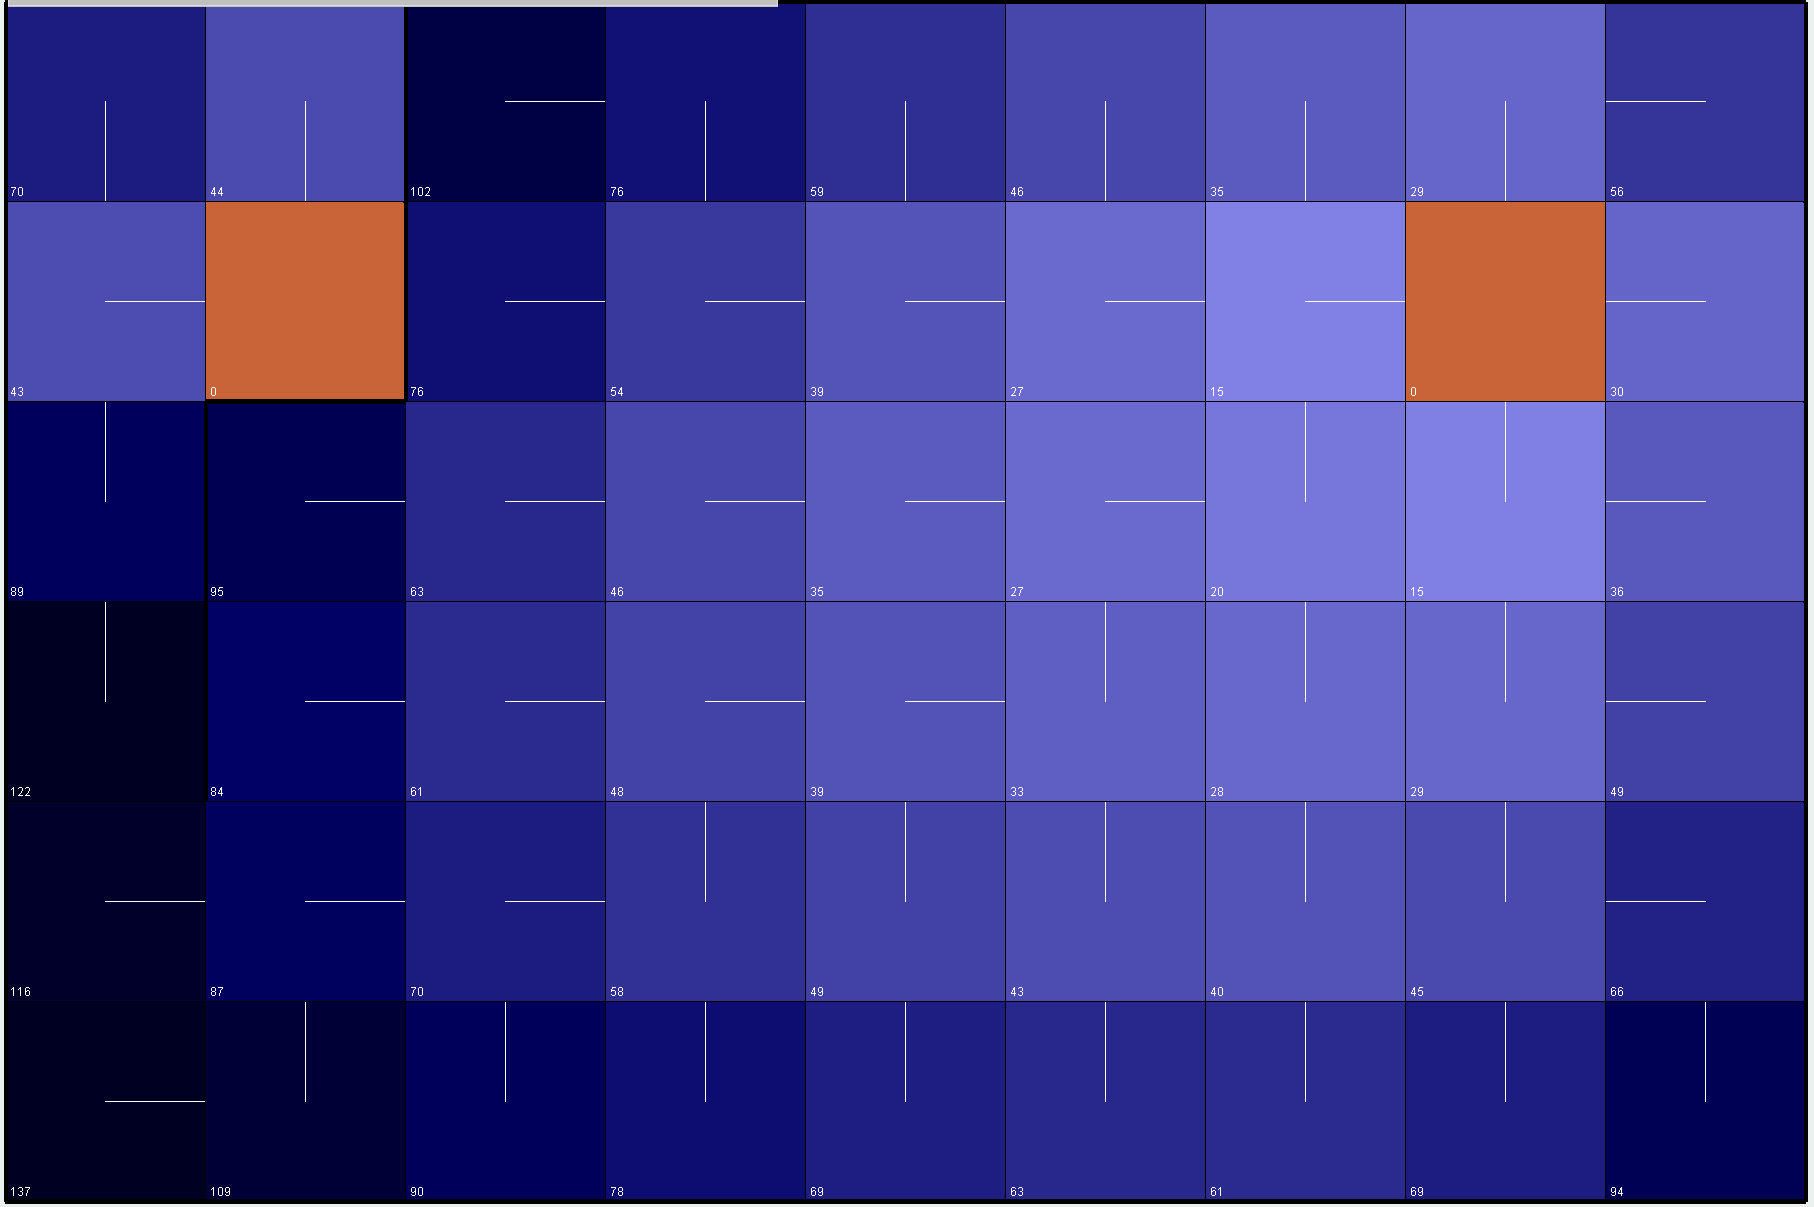
\includegraphics[width=1.2\linewidth]{../figures/value1_5.png}
     \caption{Small Maze, Value Iteration, PJOG=0.5}\label{Fig:value1_5}
   \end{minipage}\hfill
   \begin{minipage}{0.4\textwidth}
     \centering
     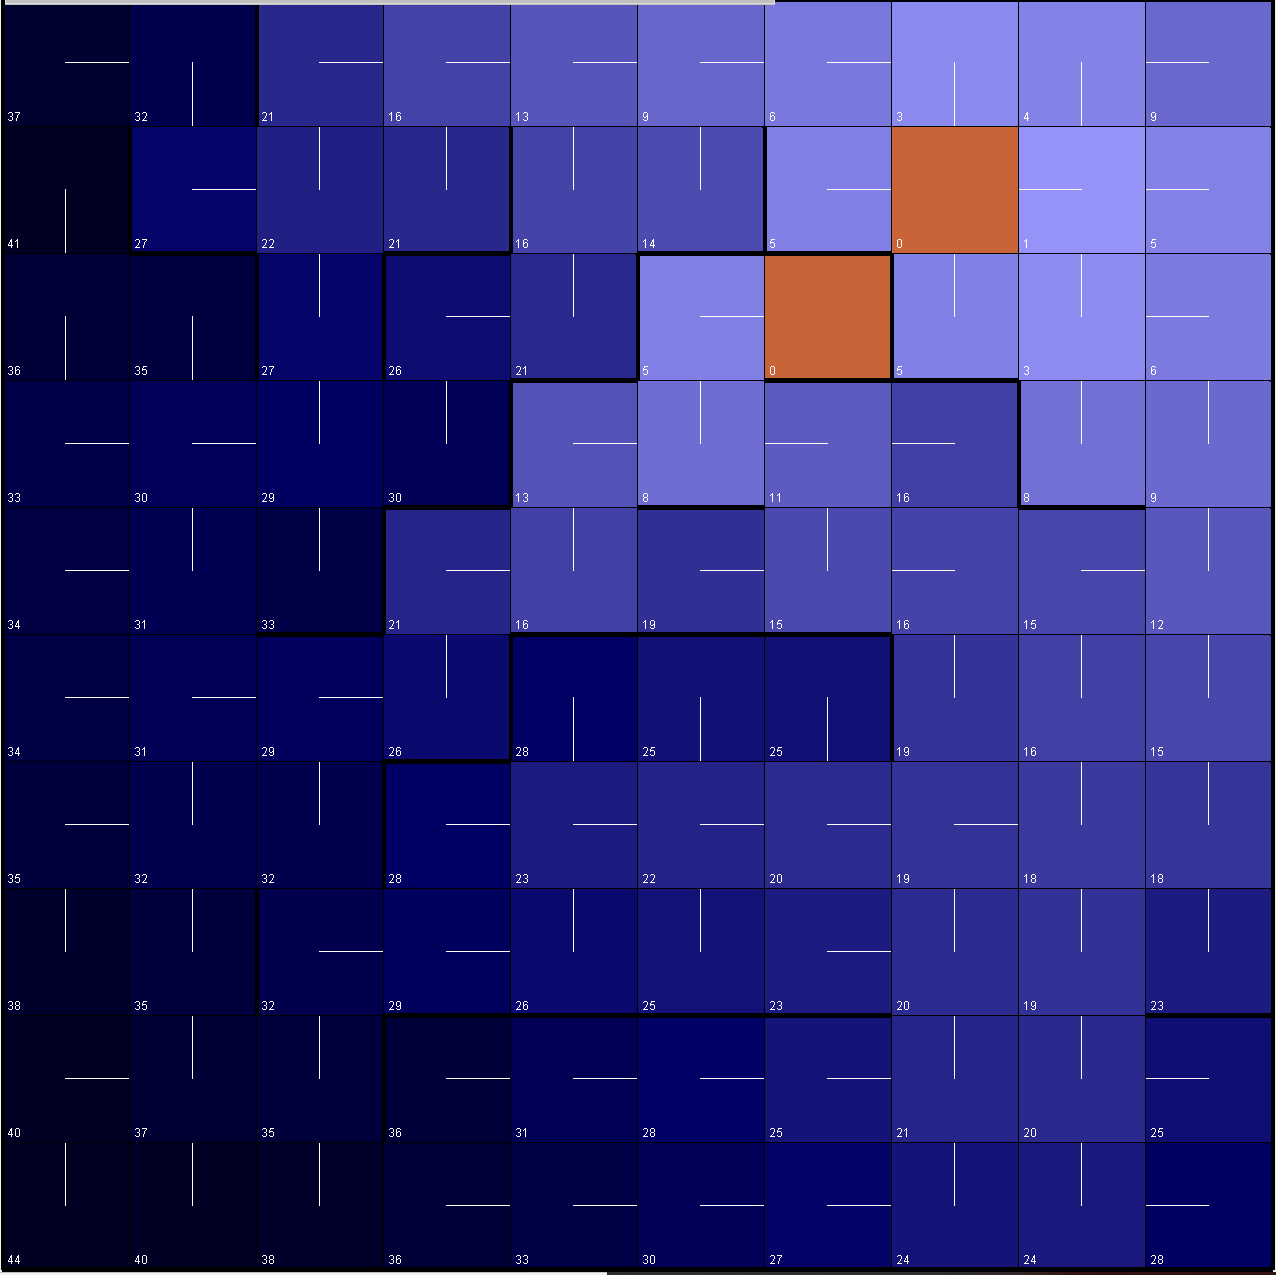
\includegraphics[width=1.2\linewidth]{../figures/value2_1.png}
     \caption{Large Maze, Value Iteration, PJOG=0.1}\label{Fig:value2_1}
   \end{minipage}
\end{figure}

\begin{figure}[!htb]
   \begin{minipage}{0.4\textwidth}
     \centering
     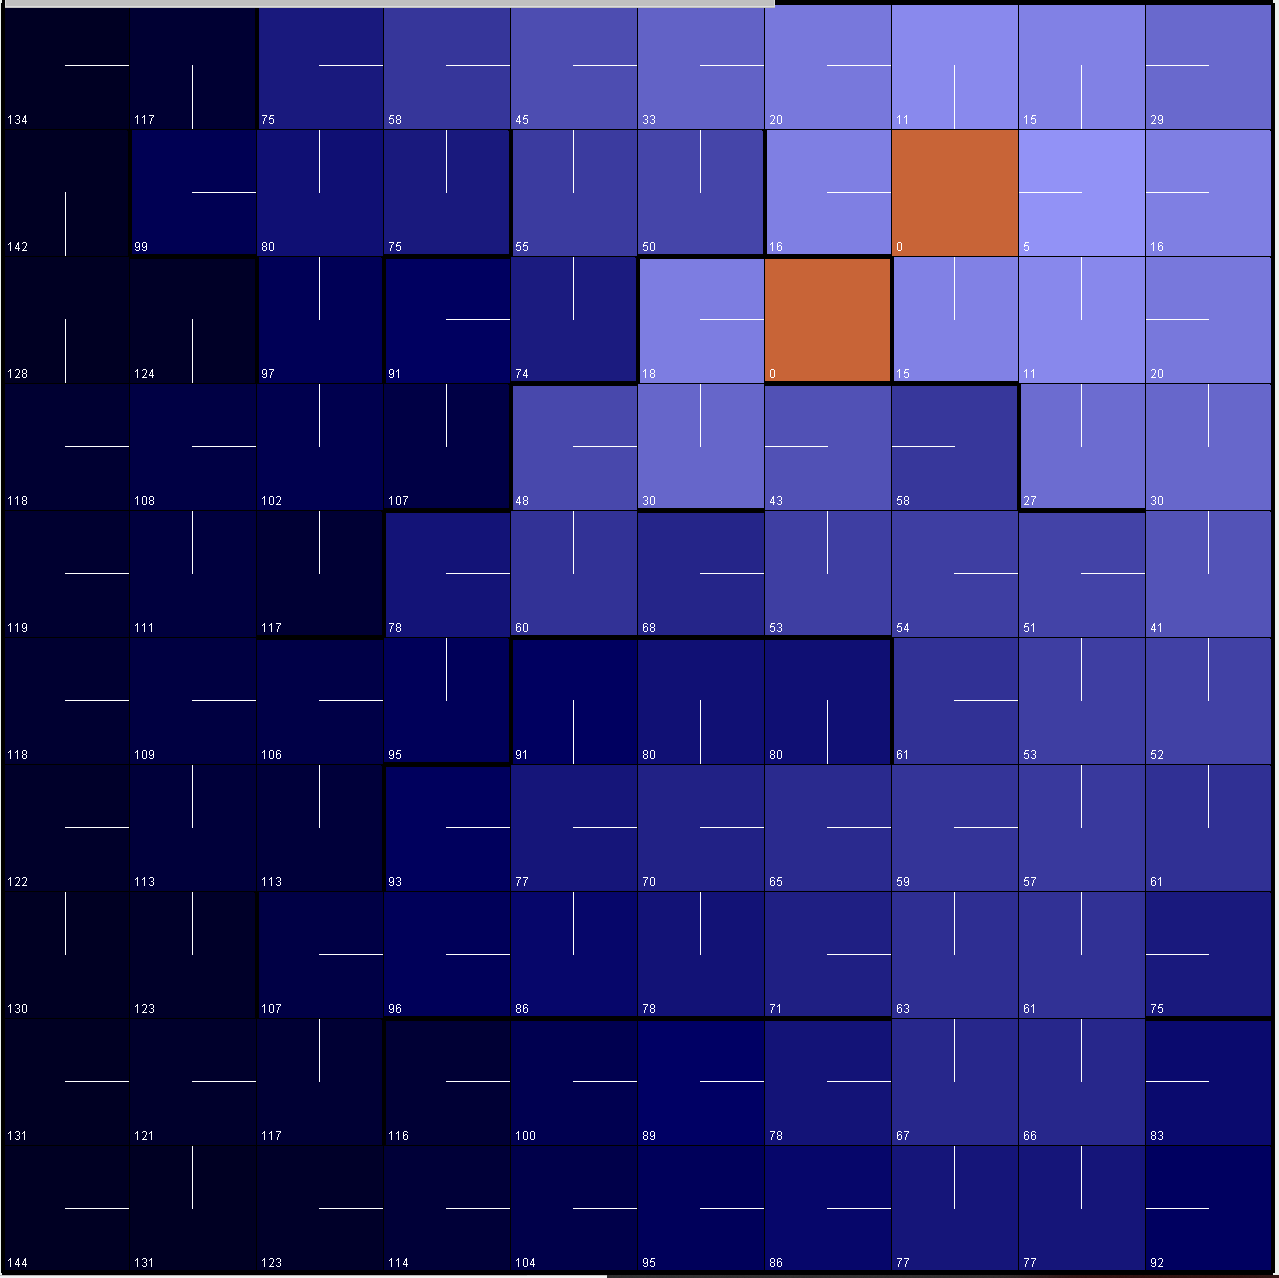
\includegraphics[width=1.2\linewidth]{../figures/value2_3.png}
     \caption{Large Maze, Value Iteration, PJOG=0.3}\label{Fig:value2_3}
   \end{minipage}\hfill
   \begin{minipage}{0.4\textwidth}
     \centering
     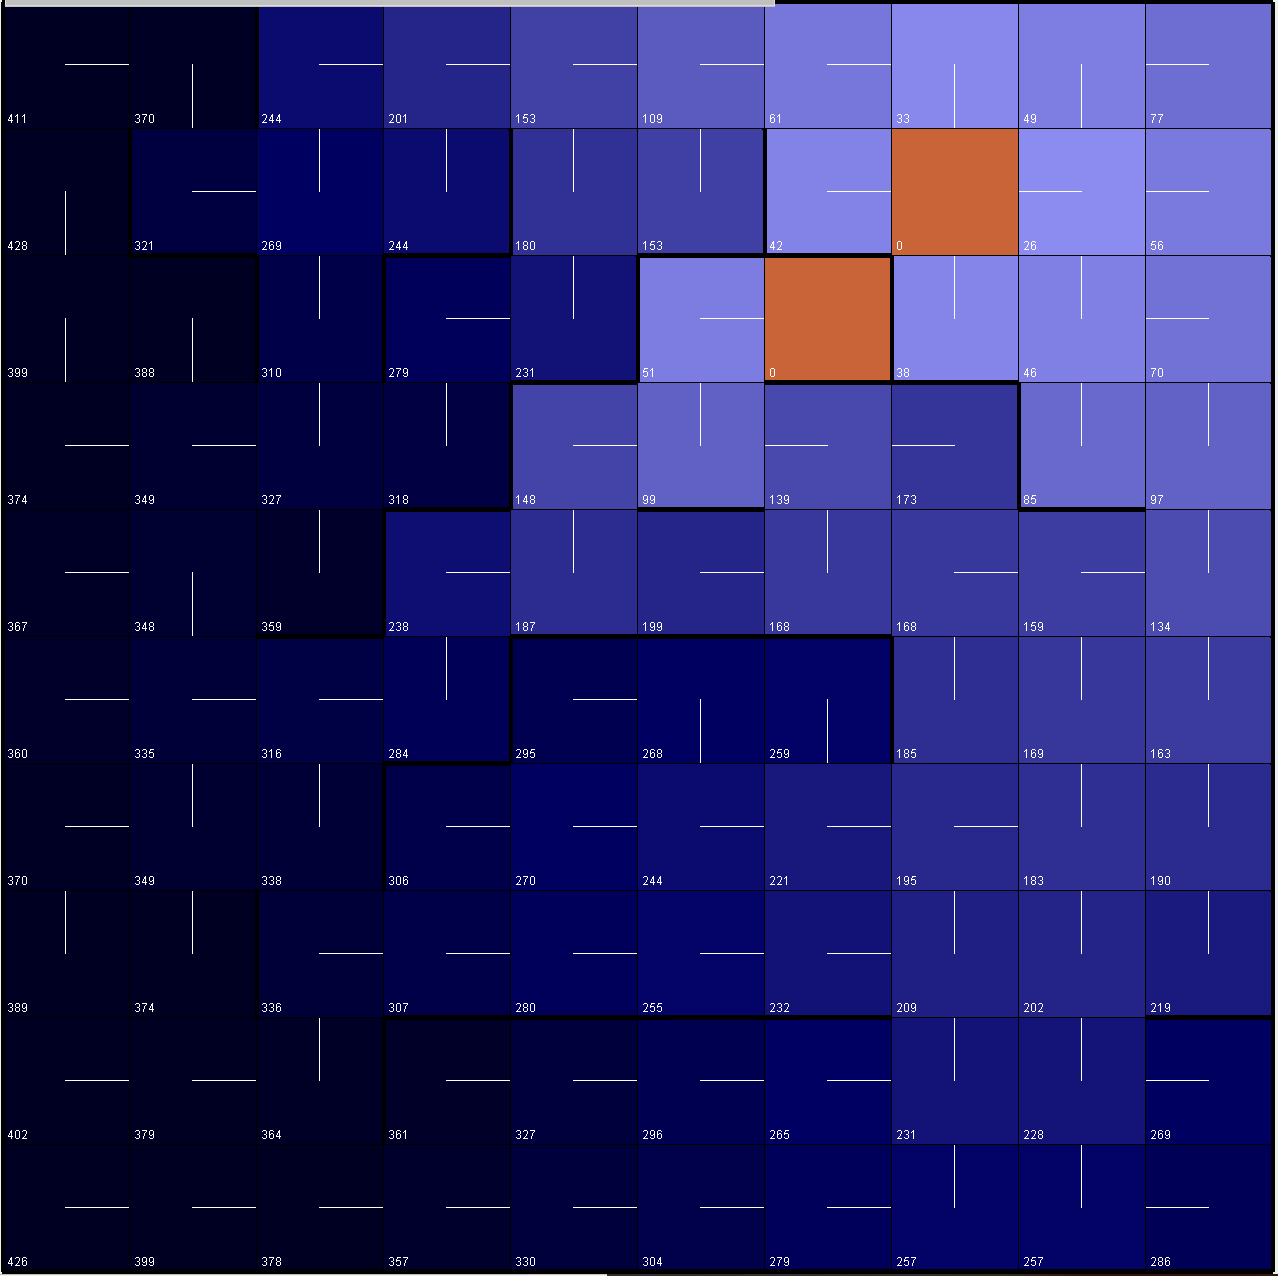
\includegraphics[width=1.2\linewidth]{../figures/value2_5.png}
     \caption{Large Maze, Value Iteration, PJOG=0.5}\label{Fig:value2_5}
   \end{minipage}
\end{figure}

\section{Policy Iteration}
For policy iteration,  it performs two steps in each iteration. First is policy evaluation, it is going to apply the Bellman operator for the current best policy in a recursive manner until convergence to the value function for the policy. Then, it will do policy improvement by taking the action that maximizes the value function for every state. \ref{Tab:policy} shows the time and steps for value iteration to converge for different selection of PJOG value. Fig.\ref{Fig:policy1_1} to Fig.\ref{Fig:policy1_5} shows the result of small maze and Fig.\ref{Fig:policy2_1} to Fig.\ref{Fig:policy2_5} shows the result of large maze.

\begin{table}[h!]
  \begin{center}
    \caption{Performance of Policy Iteration}
    \label{Tab:policy}
    \begin{tabular}{c|c|c|c|c}
			\textbf{PJOG} & \textbf{Small\_Iterations} & \textbf{Small\_Time(ms)} & \textbf{Large\_Iterations} & \textbf{Large\_Time(ms)}\\
      \hline
      0.1 & 5 & 40 & 6 & 92\\
      0.3 & 4 & 13 & 7 & 69\\
      0.5 & 4 & 24 & 5 & 100\\
    \end{tabular}
  \end{center}
\end{table}
From the experiments, we can see that it always takes small iterations for policy iteration to converge. An interesting observation is that when PJOG is equal to 0.1, it will take much time to converge, compared with the case when PJOG is 0.3. For small maze, it even takes more time when PJOG is 0.5. 

\begin{figure}[!htb]
   \begin{minipage}{0.4\textwidth}
     \centering
     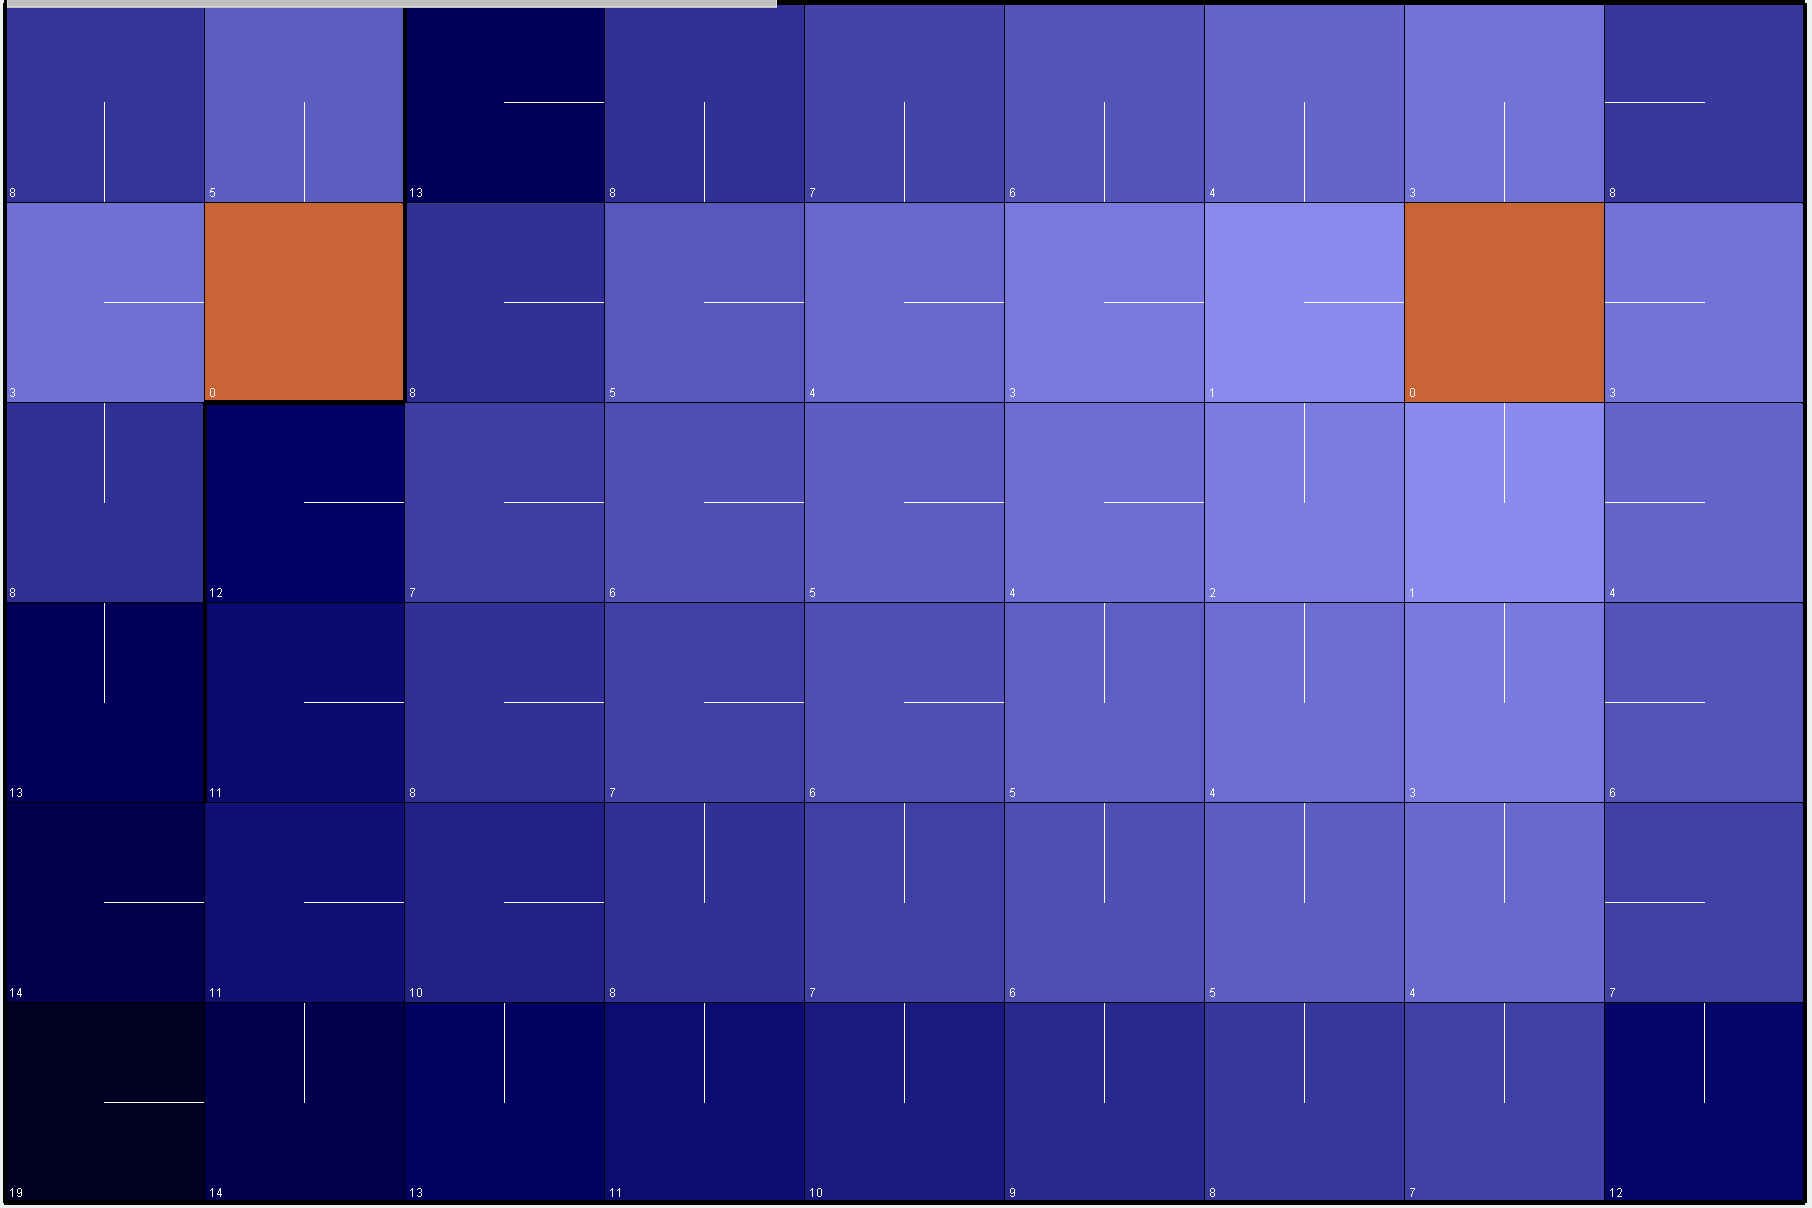
\includegraphics[width=1.2\linewidth]{../figures/policy1_1.png}
     \caption{Small Maze, Policy Iteration, PJOG=0.1}\label{Fig:policy1_1}
   \end{minipage}\hfill
   \begin{minipage}{0.4\textwidth}
     \centering
     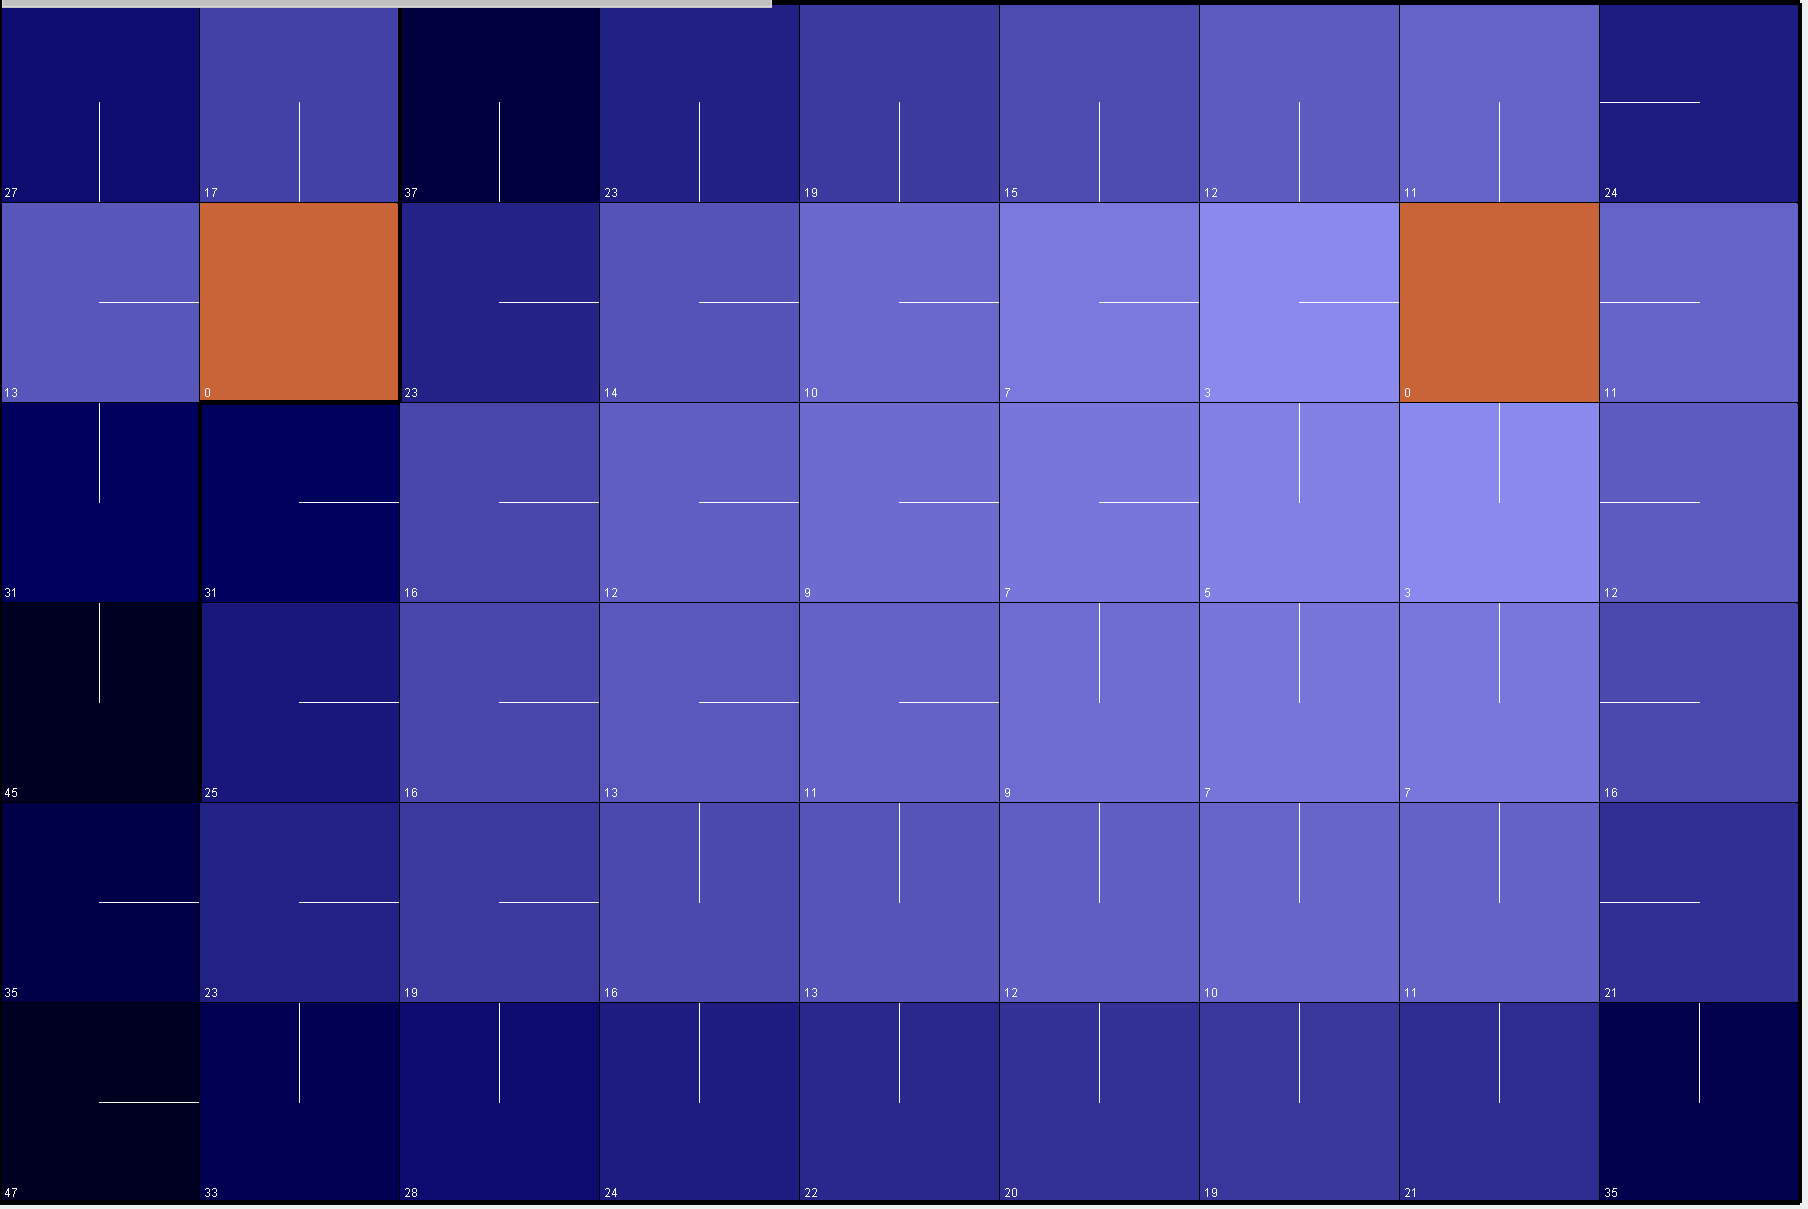
\includegraphics[width=1.2\linewidth]{../figures/policy1_3.png}
     \caption{Small Maze, Policy Iteration, PJOG=0.3}\label{Fig:value1_3}
   \end{minipage}
\end{figure}

\begin{figure}[!htb]
   \begin{minipage}{0.4\textwidth}
     \centering
     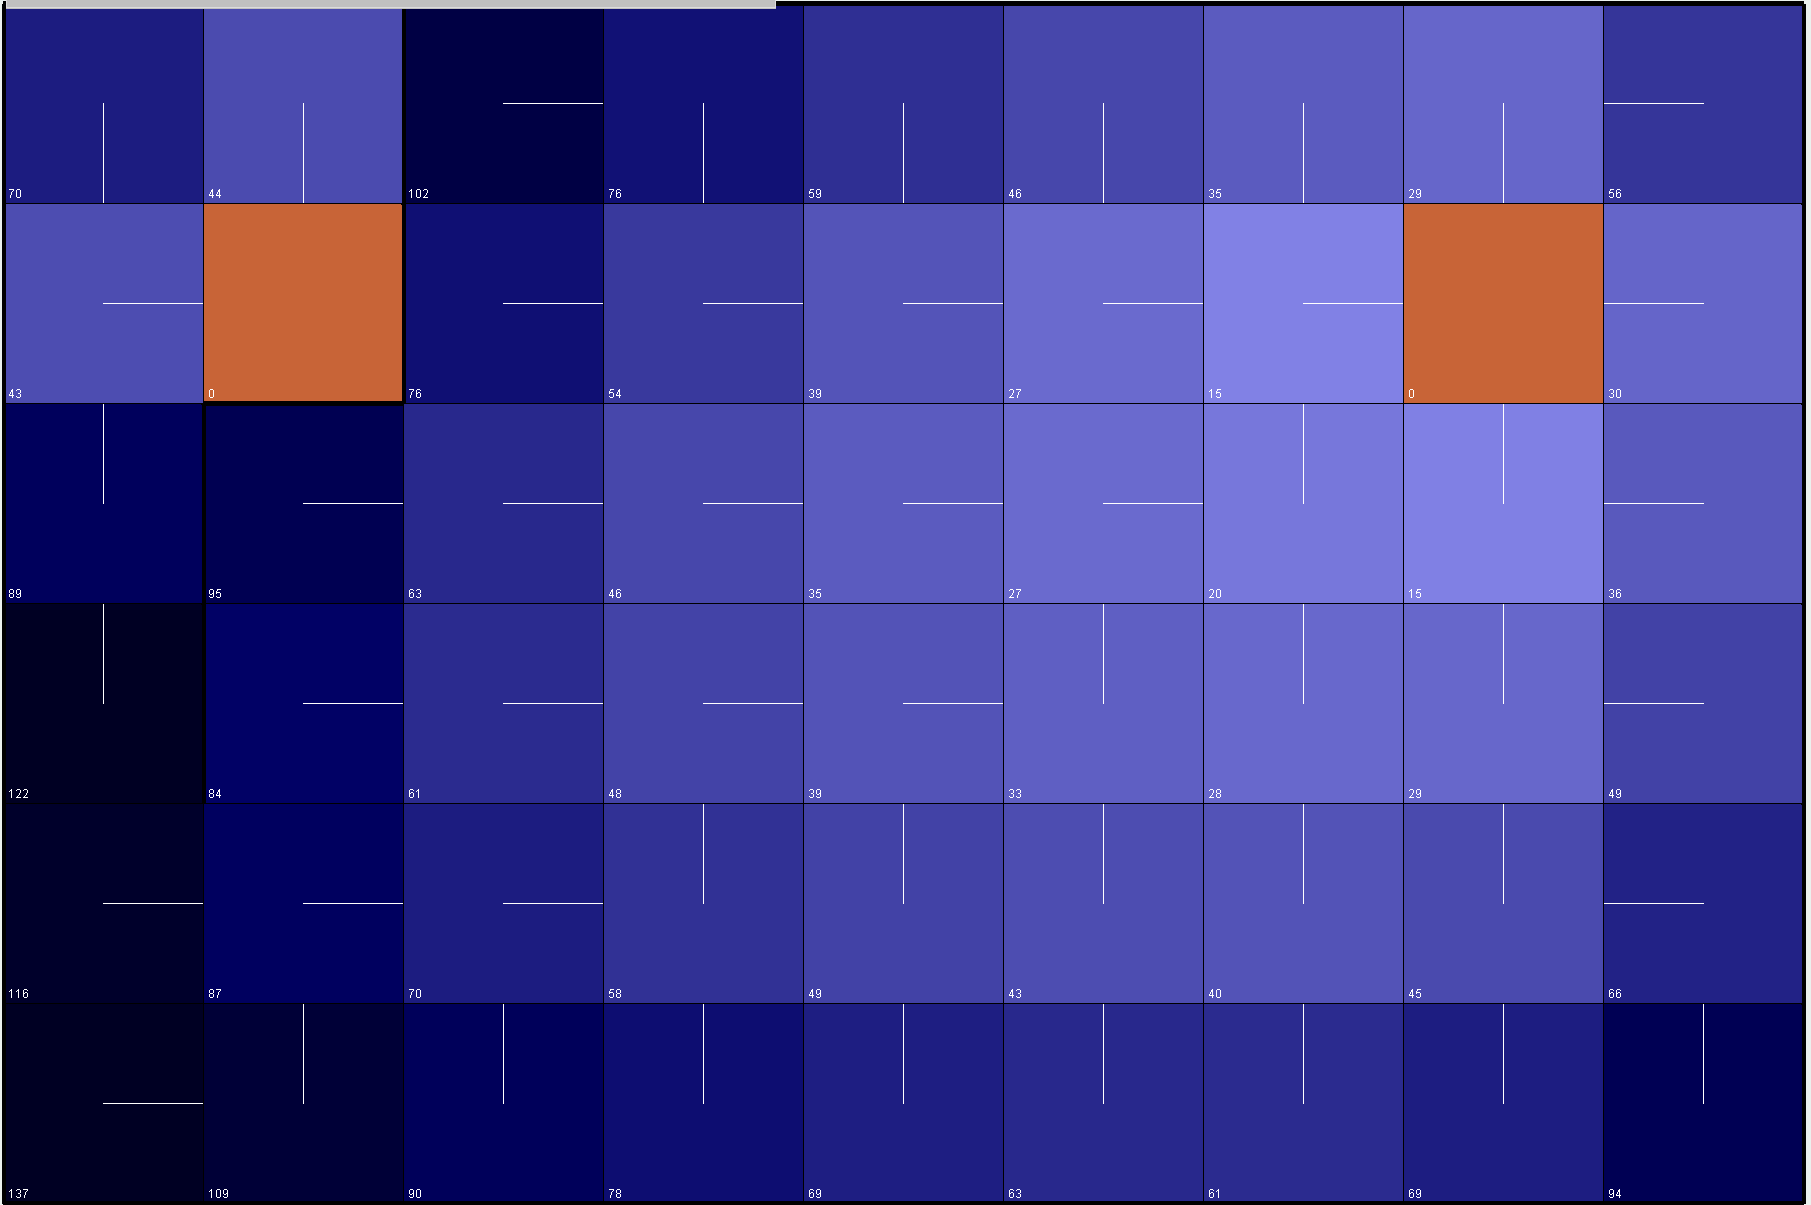
\includegraphics[width=1.2\linewidth]{../figures/policy1_5.png}
     \caption{Small Maze, Policy Iteration, PJOG=0.5}\label{Fig:policy1_5}
   \end{minipage}\hfill
   \begin{minipage}{0.4\textwidth}
     \centering
     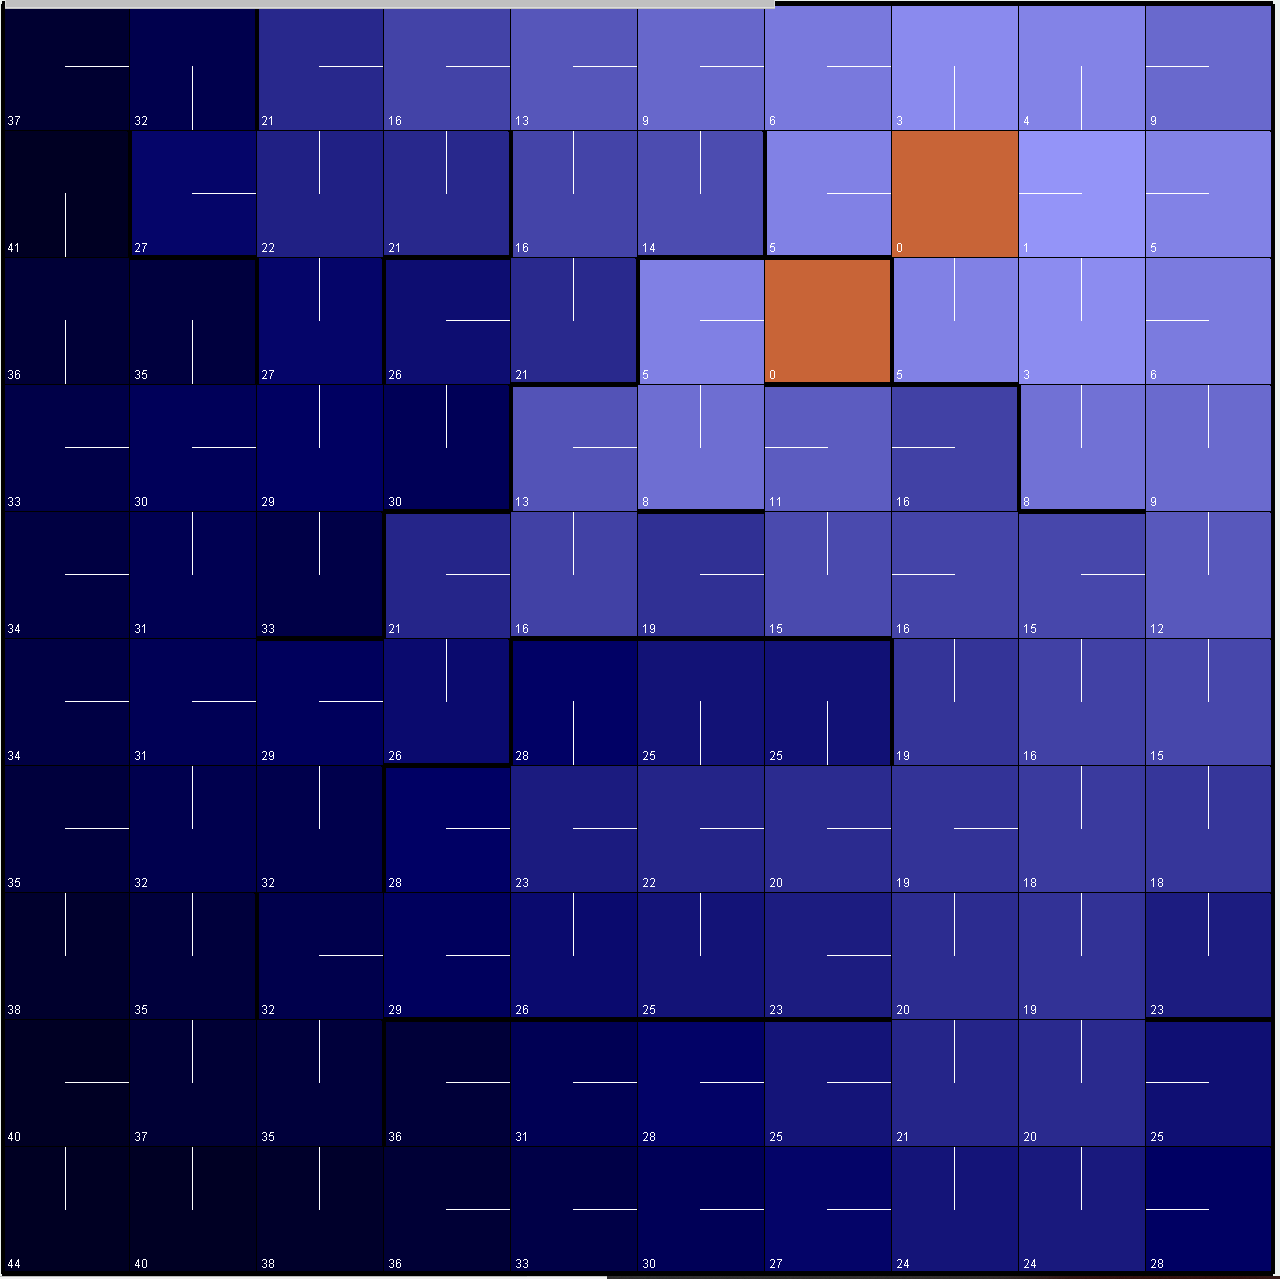
\includegraphics[width=1.2\linewidth]{../figures/policy2_1.png}
     \caption{Large Maze, Policy Iteration, PJOG=0.1}\label{Fig:policy2_1}
   \end{minipage}
\end{figure}

\begin{figure}[!htb]
   \begin{minipage}{0.4\textwidth}
     \centering
     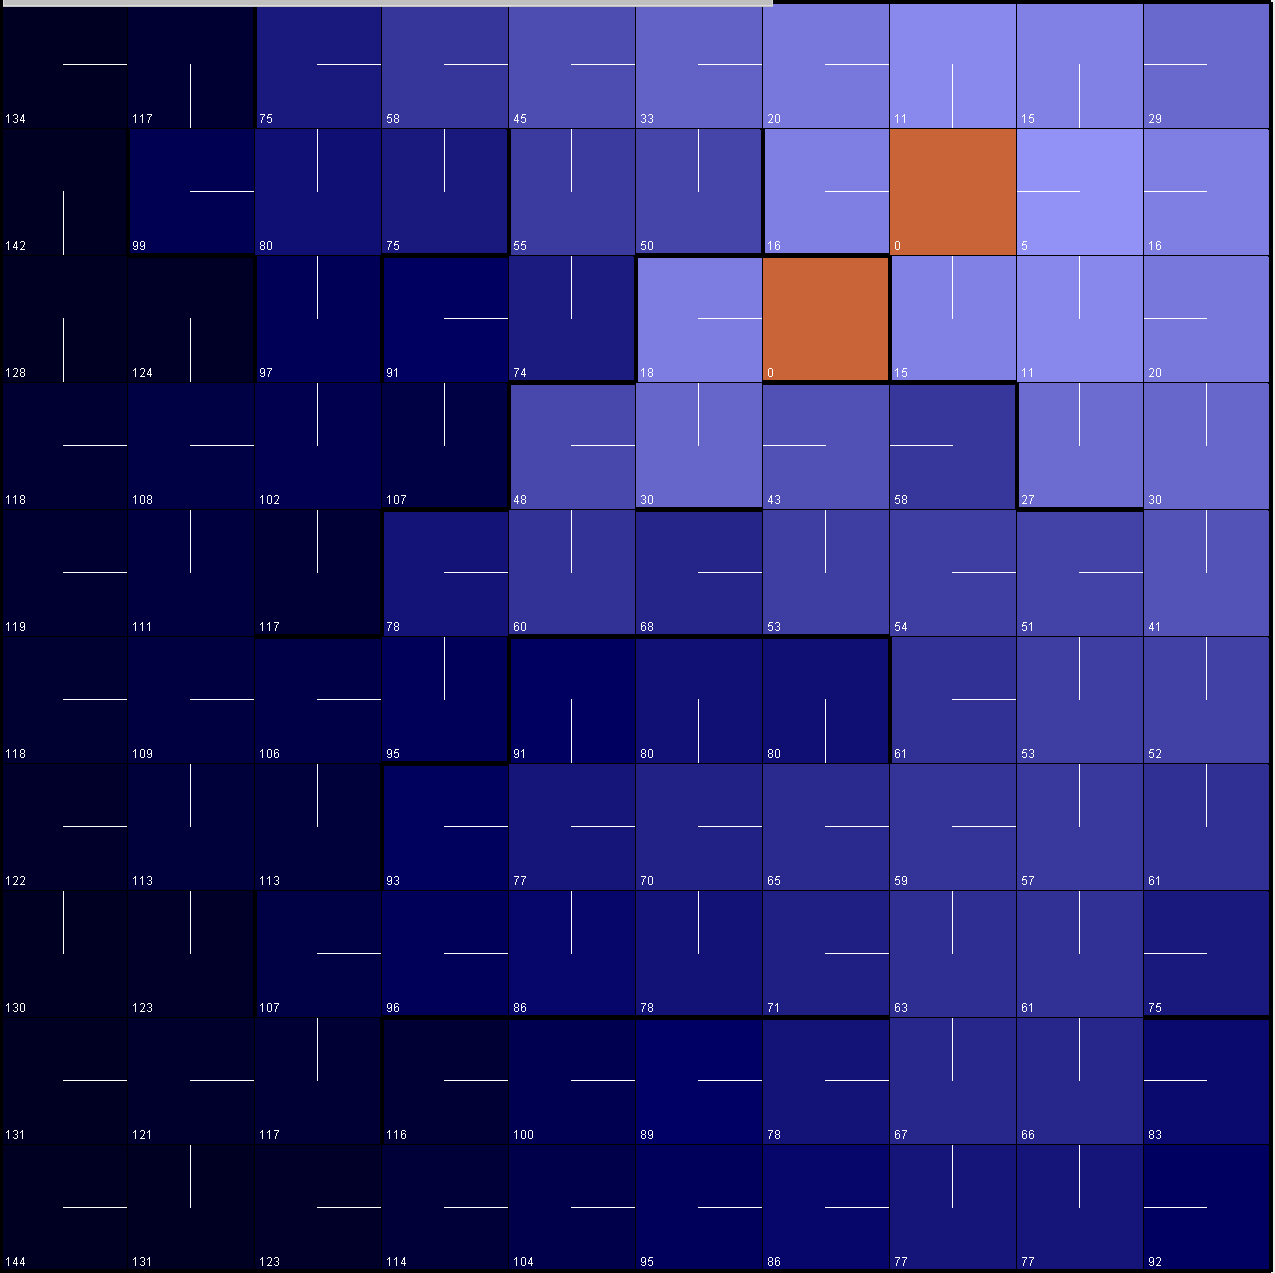
\includegraphics[width=1.2\linewidth]{../figures/policy2_3.png}
     \caption{Large Maze, Policy Iteration, PJOG=0.3}\label{Fig:policy2_3}
   \end{minipage}\hfill
   \begin{minipage}{0.4\textwidth}
     \centering
     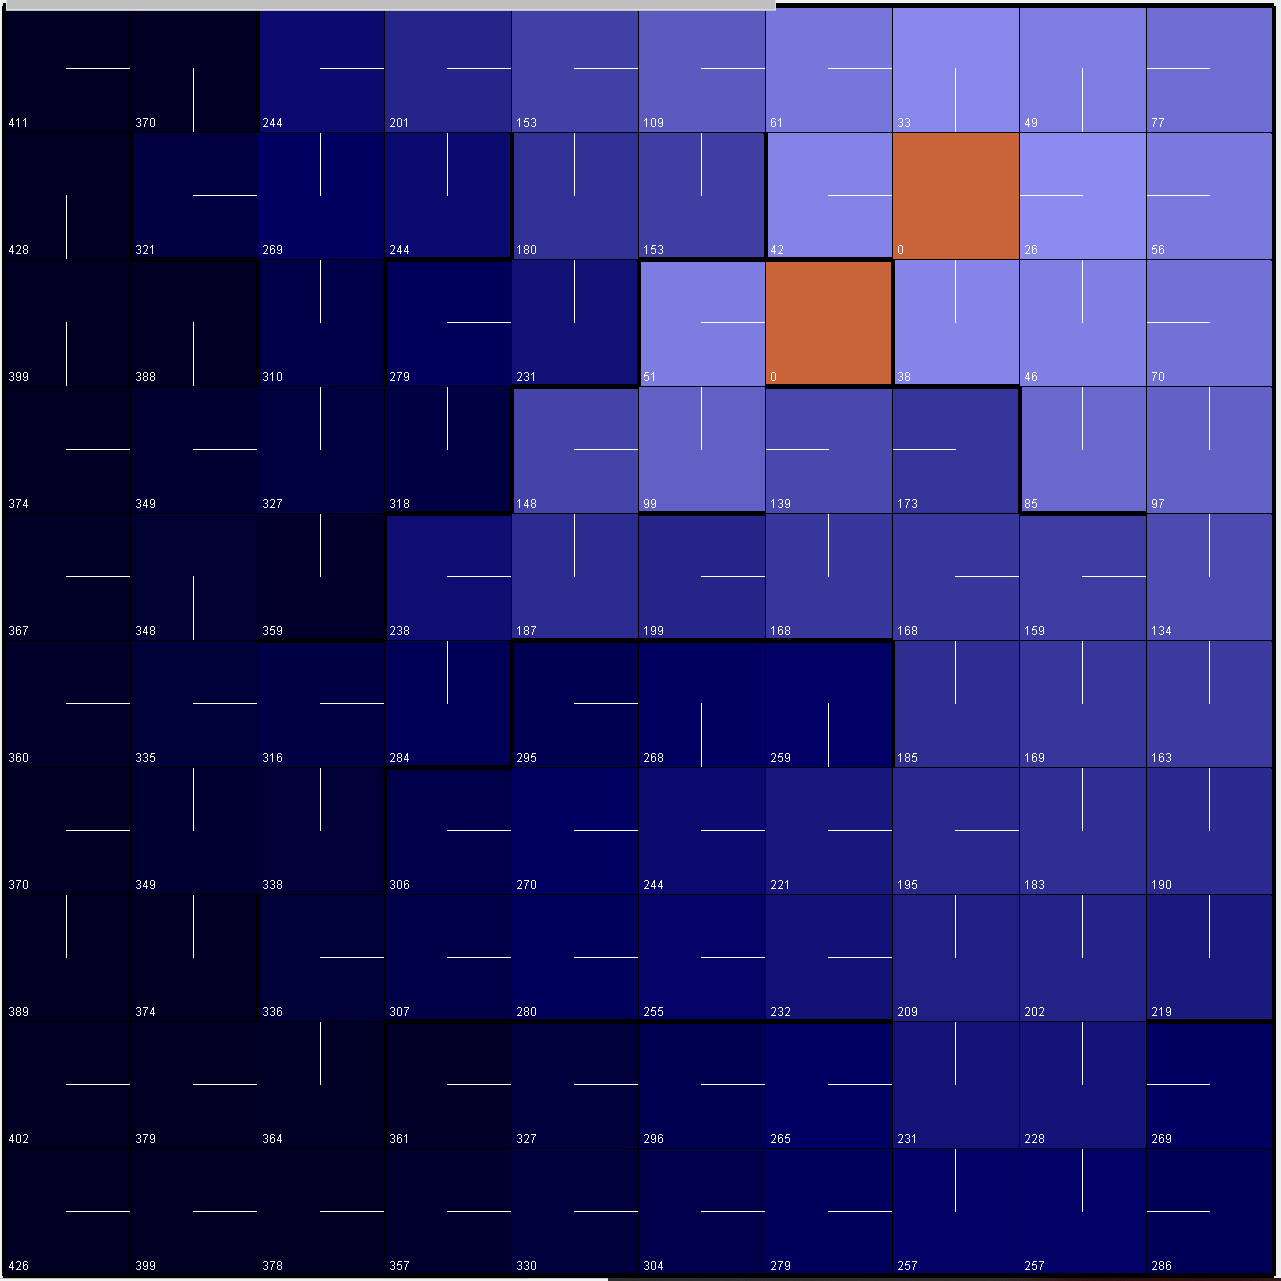
\includegraphics[width=1.2\linewidth]{../figures/policy2_5.png}
     \caption{Large Maze, Policy Iteration, PJOG=0.5}\label{Fig:policy2_5}
   \end{minipage}
\end{figure}

\section{Comparison between Value Iteration and Policy Iteration}
When we look at the results of value iteration and policy iteration, we can figure out that the results are the same. It means that both the two methods will converge to the same optimal value. Iteration steps vary a lot between value iteration and policy iteration. Policy iteration will take much smaller iterations steps to converge. This is because policy iteration is actually a kind of improvement of value iteration. Instead of waiting for convergence, we could now tolerate some error, evaluate the policy at some point and perform policy improvement over the not perfect value function. So one iteration in policy iteration is as powerful as multiple iterations in value iteration and the total iteration steps of policy iteration are consequently much smaller than that of value iteration.\\
\\
As for the convergence time, for the large maze, it is clear that when PJOG is a small value, value iteration is faster than policy iteration while policy iteration takes less time when PJOG is large. For the small maze, value iteration is smaller than policy iteration when PJOG is small and the convergence time become closer when PJOG increases. The observation indicates that policy iteration is a better choice when the problem is more complex and the agent cannot guarantee effect action. If the problem is simple or the action has a higher probability to be effective, value iteration may be quicker to converge.

\section{Q Learning}
Value iteration and policy iteration are both dynamic programming strategies, they can be used for offline planning where we make the assumption that the agent has prior knowledge about the effects of its actions on the environment. Now, assume the agent does not have prior knowledge of the system. i.e. the state transition and reward models are not known and the agent only know the possible states as well as actions.  Q learning is an example of model-free learning algorithm, the agent will discover the environment and learn the transition and reward model. It works by estimating the vale of state-action pairs. The agent initialize the pairs using arbitrary values and by observing the reward and state transition of its action, it can update the estimation of state-action pairs. A problem here is how the agent select actions during learning. The approach used is $\epsilon$-greedy approach where the agent will explore by picking random actions with probability $\epsilon$ or select an action based on the current estimate of Q values with probability $1-\epsilon$.


\end{document}
